% !TEX program = pdflatex

\section{Assigment 2}

\subsection{The Client}
The client of the project is a medium size hotel in China, the Jason Hotel.

\subsection{The Task to be Undertaken}
Our project aims to help hotel receptionists in their work, making easier and quicker for them to book rooms for the hotel's guests. 

The software will allow them to book a rooms in few clicks, to find out precisely and immediately which rooms are free and for how many days, the general availiability of rooms in a certain period, the features of every room and so on. 

It will also help the hotel owner while billing the clients, calculating automatically the price of the stay and the total revenue of the hotel in a certain period.

We will develop our software on three sides: realizing a database containing the information about hotel's rooms and their availiability, designing a graphical interface that will be user-friendly to minimize the training period of the staff and allow them to be comfortable with our software, and developing a software that will hold database's informations for the staff and help the owner to bill clients and to calculate the revenue of his hotel.

\subsection{Requirement Analysis}

The system will meet the following requirements.

\subsubsection{Interface}

\begin{enumerate}
	
\item Booking Interface
    \begin{itemize}
		\item Intuitive and user-friendly to provide a quick answer to the client for his request, and if possible, confirm with one click the booking.
		\item Has a section where fill the date of check-in and check-out and show all the rooms free for that period. The system can show many type of rooms and prices.
		\item Has some feature to satisfy other request, like guest disability, pet, child, smoker. For example, for a disable guest the system choose a room at the lower floor possible
		\item Has a form for fill the guest information, like name, passport, e-mail. If the guest can't give all the information immediately can be filled later in the room section
    \end{itemize}
	
\item Rooms interface
    \begin{itemize}
		\item Has a section where see all the room, if they are free or occupied in the current day or a choosed period.
		\item Clicking on the room the user can see all the feature of the room, and also modify it if necessary, if it's booked or occupied the system show also all the guests data.
		\item The user can modify guests data, check-in/out time or delete the booking. 
		\item A form can be filled with other particular requests, in case.
    \end{itemize}
    
\item Guest Search Interface
	\begin{itemize}
		\item Has a form to fill with the name and will return all the available information about such guest. 
	\end{itemize}

\item Billing interface
    \begin{itemize}
		\item It can be opened only by the manager with a log-in page.
		\item It shows all the revenue of the hotels for a day, week, or month.
		\item In the main page it shows the bill for all the guest which check-out is the current day.
    \end{itemize}

\end{enumerate}

\subsubsection{DataBase}
    \begin{itemize}
	\item It must be pre-filled with the hotel map, with all the rooms.
	\item It has a first table for the rooms and some column to specify rooms occupation, type and feature.
	\item It has a second table for the guests information, linked with a 1-m relation with the room (a room can have many guests, but a guest can stay in only one room)
	\item It has a third table for the revenue of the hotel.
	\item (optional) all the important information can be encrypted
    \end{itemize}
    
\subsection{Suggested Deliverables}

Not being expert on the main procedures about hotel’s organization, we believe that to realize this project a continuos and total collaboration among System Analysts, System Designers, System Developers and Final Users is crucial.

\subsubsection{Management deliverables}

Our intention is to organize many meetings and a documentation about Requirement Analysis in such a way to be sure:
\begin{enumerate}
	\item To have a complete acquaintance of clients’ necessity and expectations.
	\item To improve the communication and cooperation level among developers, designers, managers and users.
	\item To give the final user the possibility to have a central role during the entire development of the system and to choose, from time to time, the best solution.
\end{enumerate}

\subsubsection{Design Document}

We want to document and to maintain the presence of final users even in the design process of the system. 
By doing so, and by keeping in mind the Requirement Analysis, we want to meet the final users’ necessities. 
These documents will be updated for all the Design process’ duration.

\subsubsection{Source Code}

Our intention is to document all the development of the code, not only at a technical level, comprehensible only to the programmers, but even at a more user friendly level. 
So, even final users will be able to keep under control the development of the system.

\subsection{Technical deliverables}

\subsubsection{DataBase}

We are going to use a Database Structure, divided in tables, to save the different informations like:
\begin{enumerate}
	\item Rooms
	\item Guest
	\item Payments 
	\item Others
\end{enumerate}

\subsubsection{Interface}

We will organize the system as much user friendly as possible. 
We will implement the main functionalities directly on the home page. These are:
\begin{enumerate}
	\item To add / cancel a reservation.
	\item To verify the availability of a room.
	\item To verify payments.
	\item To control general services.
\end{enumerate}

\subsubsection{Interactive Structure of the Hotel}
	
According to clients’ necessity we will implement, on the home page, an interactive structure that represents the hotel. 
By doing so, final user will immediately have a complete view of general situation, and the possibility to select a room to know its details.

\subsection{Outline Plan (Principal activities and Milestones)}

\begin{enumerate}

\item (Friday 09/26) Preliminary overview of the project.

\item (Friday 10/10) Detailed system analysis, this will include:
	\begin{itemize}
		\item The task to be undertaken.
		\item The use cases.
		\item Detailed explaination of the features.
		\item The client who required the software.
	\end{itemize}

\item (Thursday 10/23) System required analysis, it will include:
  \begin{itemize}
    \item The detailed data modelling.
    \item The detailed data analysis.
    \item The detailed process modeling. 
  \end{itemize}

\item (Friday 11/07) Final describtion of the project, it will include:
  \begin{itemize}
    \item The detailed explaination of the application architecture.
    \item The detailed database design.
    \item The datailed input of the application.
    \item The detailed output of the application.
    \item The user interface design.
\end{itemize}

\end{enumerate}

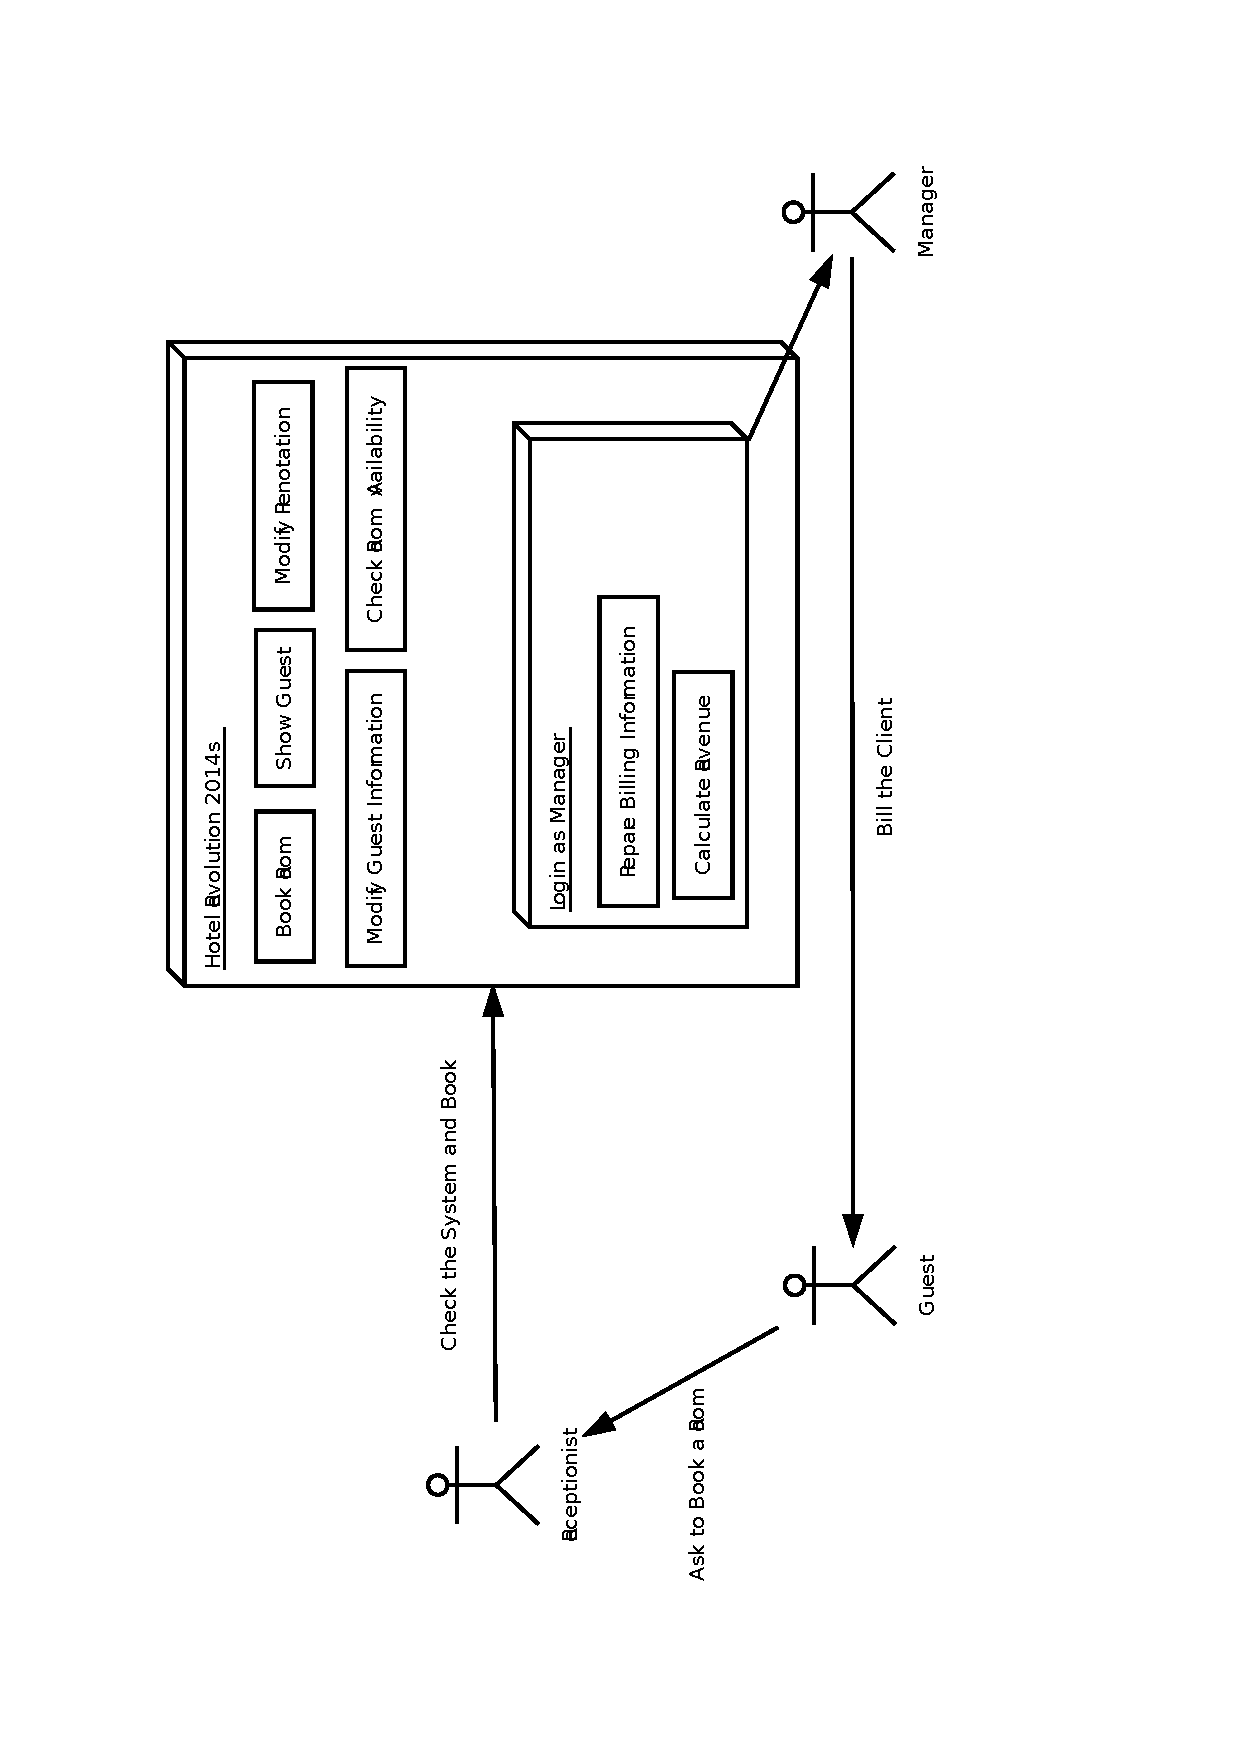
\includepdf{use-case-diagram}

\subsection{Data Model Table Attributes}

\begin{itemize}
  \item Guest \\ 
    The table contains the information about a single guest.
    \begin{itemize}
      \item GuestID: The ID for a single guest
      \item Name: The name of the guest
      \item Surname: The surname of the guest
      \item DocumentID: The ID of the document of the guest
      \item Contact: An email or a phone number to contact in case of problem
    \end{itemize}
  \item Reservation \\
    The table is necessary to manage the many-to-many relationship between Guest and Rooms.
    \begin{itemize}
      \item IDRegistration: The ID of a single reservation
      \item IDRoom: The ID of the room the guest will use for this particolar reservation
      \item IDGuest: The ID of the guest whose prenotation is refered to
      \item CheckIN: The date when the guest will arrive
      \item CheckOUT: The date when the guest will leave
    \end{itemize}    
  \item Rooms \\
    The table contains the information about the rooms in the hotel.
    \begin{itemize}
      \item IDRoom: The ID of a room
      \item RoomNumer: The number of the room in the structure
      \item PricePerNight: How much cost the room for a single night  
      \item NumGuest: The maximun number of people that room can accomodate
      \item Smoker: It is possible to smoke in the room ?
      \item WiFi: The room has WiFi access ?
    \end{itemize}
  \item User \\
    This table will keep the information about the users who can access and use the application.
    \begin{itemize}
      \item Name: Use as PrimaryKey, the username necessary to access at the application
      \item Password: The hash of the password used to access the application
      \item Manager: Is the user a manager ?
    \end{itemize}
\end{itemize}

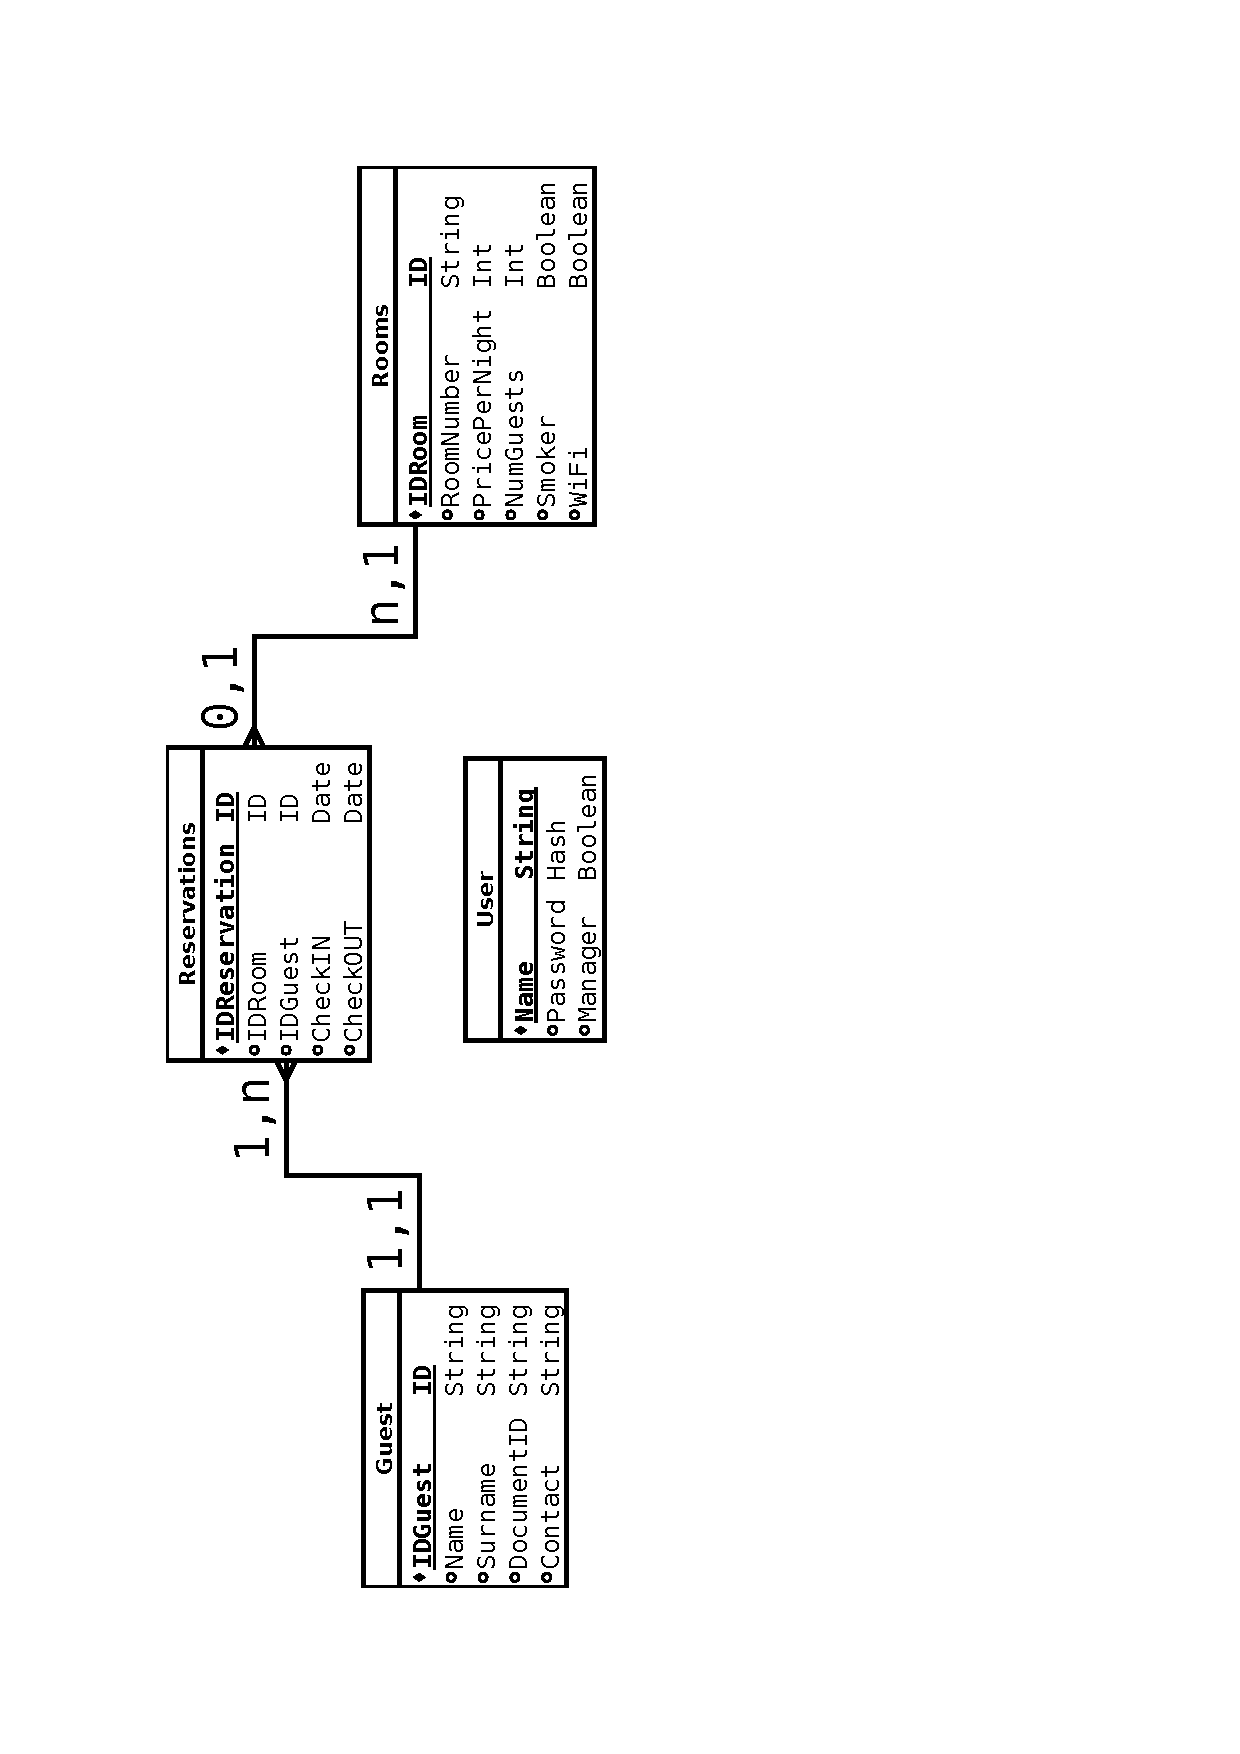
\includepdf{DataModel}

